
Hier werden analog zu 2017 die Messdaten aus dem Experiment von 2012 mit linearer Regression betrachtet.

\subsection{Prüfung auf eine einfache Abhängigkeit}

Hier werden sechs Gleichungen mittels linearer Regression ermittelt: 

\[v_{auf}(v_{ebene}) = \beta_0 + \beta_1 v_{ebene}\]
\[v_{ab}(v_{ebene}) = \beta_0 + \beta_1 v_{ebene}\]

\[v_{auf}(groesse) = \beta_0 + \beta_1 groesse\]
\[v_{ab}(groesse) = \beta_0 + \beta_1 groesse\]

\[v_{auf}(runde) = \beta_0 + \beta_1 runde\]
\[v_{ab}(runde) = \beta_0 + \beta_1 runde\]

\subsubsection{Wunschgeschwindigkeit in der Ebene}

Für die Abhängigkeit Wunschgeschwindigkeit in der Ebene wurde 
der Zusammenhang wie in den Formeln für die Treppengeschwindigkeit aufwärts (\ref{eq:auf2012-ebene}) und abwärts (\ref{eq:ab2012-ebene}) ermittelt. 

\begin{equation} \label{eq:auf2012-ebene}
	v_{auf}(v_{ebene}) = -2.13306 + 1.92532 v_{ebene}
\end{equation}
\begin{equation} \label{eq:ab2012-ebene}
	v_{ab}(v_{ebene}) = -1.05942 + 1.28244 v_{ebene}
\end{equation}

Beide Steigungen sind positiv. Hat ein Proband eine schnellere Wunschgeschwindigkeit in der Ebene, verhält er sich auch schneller auf 
der Treppe. Die Abbildungen \ref{fig:auf2012-ebene} und \ref{fig:ab2012-ebene}
stellen dies grafisch dar. 

\begin{figure} \centering 
	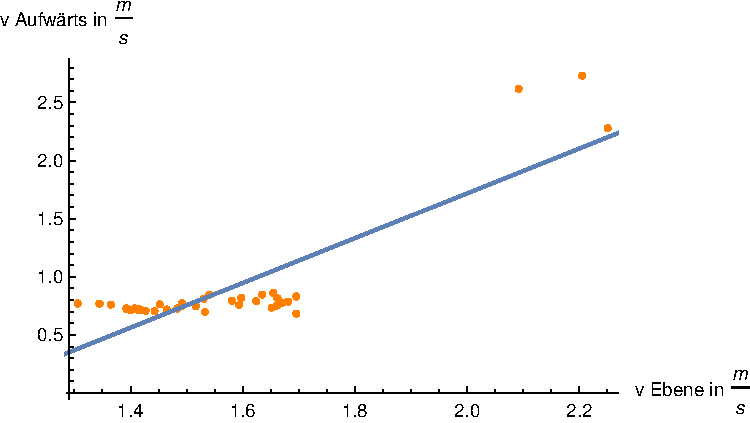
\includegraphics[]{abbildungen/regression/2012/auf-ebene.pdf}
	\[\begin{array}{l|llll}
 \text{} & \text{Estimate} & \text{Standard Error} & \text{t-Statistic} & \text{P-Value} \\
\hline
 1 & 0.506746 & 0.0900029 & 5.63033 & \text{2.603647901106944$\grave{ }$*${}^{\wedge}$-6} \\
 \text{vEbene} & 0.168071 & 0.0588553 & 2.85567 & 0.00727064 \\
\end{array}\]


	\caption{Abhängigkeit Wunschgeschwindigkeit in der Ebene zur Treppengeschwindigkeit aufwärts. Messdaten (orange) mit ermittelter Regressionsgerade (blau). \label{fig:auf2012-ebene}}
\end{figure}

\begin{figure} \centering 
	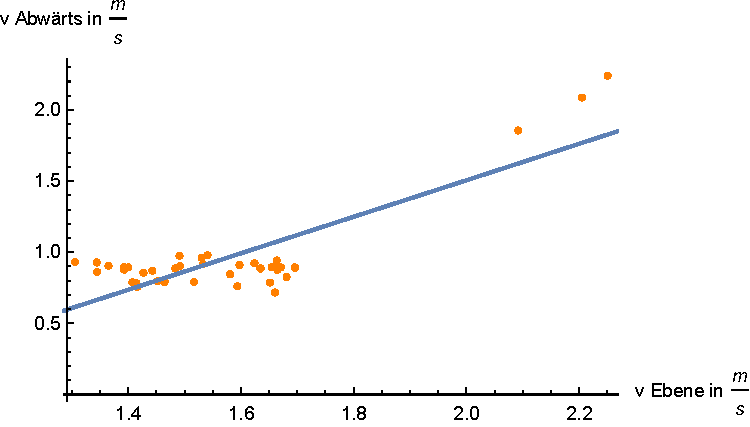
\includegraphics[]{abbildungen/regression/2012/ab-ebene.pdf}
	\[\begin{array}{l|llll}
 \text{} & \text{Estimate} & \text{Standard Error} & \text{t-Statistic} & \text{P-Value} \\
\hline
 1 & 0.440848 & 0.213068 & 2.06904 & 0.0428577 \\
 \text{vEbene} & 0.478525 & 0.142985 & 3.34668 & 0.00141579 \\
\end{array}\]


	\caption{Abhängigkeit Wunschgeschwindigkeit in der Ebene zur Treppengeschwindigkeit abwärts. Messdaten (orange) mit ermittelter Regressionsgerade (blau). \label{fig:ab2012-ebene}}
\end{figure}

In Abbildung \ref{fig:auf2012-ebene} sind wieder Ausreißer zu erkennen. In 2012 sind die Ausreißer (Datensätze mit Bemerkung) viel stärker ausgeprägt. Es ergeben sich neue Formeln für die Treppengeschwindigkeit aufwärts (\ref{eq:ohne-auf2012-ebene}) und abwärts (\ref{eq:ohne-ab2012-ebene}). Dazu gehören Abbildungen \ref{fig:ohne-auf2012-ebene} und \ref{fig:ohne-ab2012-ebene}.
Zur Vergleichbarkeit wurden aber dennoch in den weiteren Regressionen alle Daten (mit Ausreißern) verwendet.


\begin{equation} \label{eq:ohne-auf2012-ebene}
	v'_{auf}(v_{ebene}) = 0.506746 + 0.168071  v_{ebene}
\end{equation}
\begin{equation} \label{eq:ohne-ab2012-ebene}
	v'_{ab}(v_{ebene}) = 0.875577 - 0.00429171 v_{ebene}
\end{equation}

\begin{figure} \centering 
	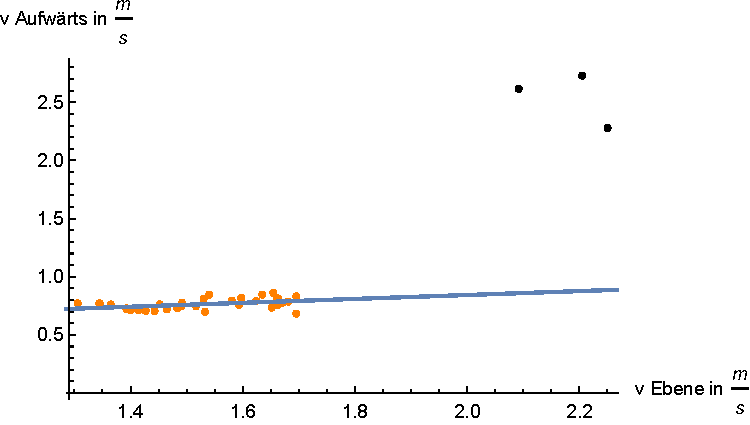
\includegraphics[]{abbildungen/regression/2012/ohneausreisser/auf-ebene.pdf}
	\[\begin{array}{l|llll}
 \text{} & \text{Estimate} & \text{Standard Error} & \text{t-Statistic} & \text{P-Value} \\
\hline
 1 & 0.506746 & 0.0900029 & 5.63033 & \text{2.603647901106944$\grave{ }$*${}^{\wedge}$-6} \\
 \text{vEbene} & 0.168071 & 0.0588553 & 2.85567 & 0.00727064 \\
\end{array}\]


	\caption{Abhängigkeit Wunschgeschwindigkeit in der Ebene zur Treppengeschwindigkeit aufwärts. Gefilterte Messdaten (orange) und Ausreißer (schwarz) mit ermittelter Regressionsgerade (blau). \label{fig:ohne-auf2012-ebene}}
\end{figure}

\begin{figure} \centering 
	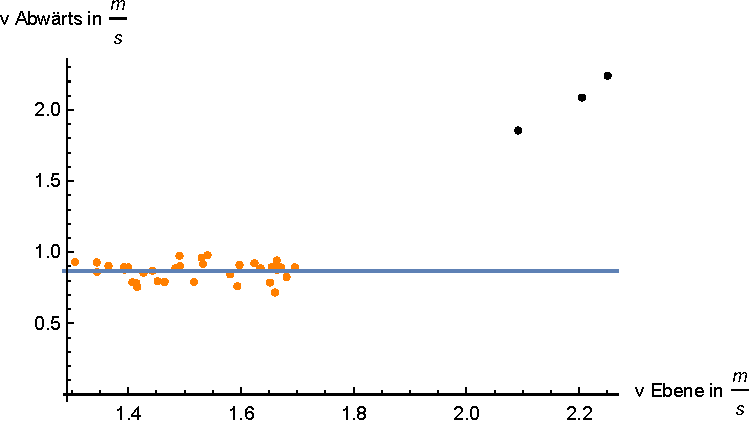
\includegraphics[]{abbildungen/regression/2012/ohneausreisser/ab-ebene.pdf}
	\[\begin{array}{l|llll}
 \text{} & \text{Estimate} & \text{Standard Error} & \text{t-Statistic} & \text{P-Value} \\
\hline
 1 & 0.440848 & 0.213068 & 2.06904 & 0.0428577 \\
 \text{vEbene} & 0.478525 & 0.142985 & 3.34668 & 0.00141579 \\
\end{array}\]


	\caption{Abhängigkeit Wunschgeschwindigkeit in der Ebene zur Treppengeschwindigkeit abwärts. Gefilterte Messdaten (orange) und Ausreißer (schwarz) mit ermittelter Regressionsgerade (blau).
	\label{fig:ohne-ab2012-ebene}}
\end{figure}

Für die Plausibilisierung der Regression wird die Nullhypothese 
$H_0: \beta_1 = 0$ aufgestellt. Signifikanzniveau $\alpha = 0.05$.
Die Ergebnisse des Tests sind in Abbildung \ref{fig:auf2012-ebene} zu sehen.
Signifikanz liegt vor, weil $p < \alpha$. Man verwirft die
Nullhypothese. Kein Einfluss von $v_{ebene}$ auf $v_{auf}$ wäre unplausibel, wenn auch nicht ausgeschlossen.

Die Nullhypothese und das Signifikanzniveau sind für alle folgenden Regressionen gleich. Die Ergebnisse für den Abstieg sind in Abbildung \ref{fig:ab2012-ebene} zu sehen.
Signifikanz liegt vor, weil $p < \alpha$. Man verwirft die
Nullhypothese. Kein Einfluss von $v_{ebene}$ auf $v_{ab}$ wäre unplausibel, wenn auch nicht ausgeschlossen.

\subsubsection{Körpergröße}

Für die Abhängigkeit Körpergröße wurde 
der Zusammenhang (\ref{eq:auf2012-groesse}) und (\ref{eq:ab2012-groesse}) ermittelt.

\begin{equation} \label{eq:auf2012-groesse}
	v_{auf}(groesse) = 2.428 - 0.00854845 groesse
\end{equation}
\begin{equation} \label{eq:ab2012-groesse}
	v_{ab}(groesse) = 2.20944 - 0.00698501 groesse
\end{equation}

In den Abbildungen \ref{fig:auf2012-groesse} und \ref{fig:ab2012-groesse} ist 
zu sehen, dass sich nach dem Modell größere Personen egal ob aufwärts oder abwärts langsamer auf der Treppe bewegen.

\begin{figure} \centering 
	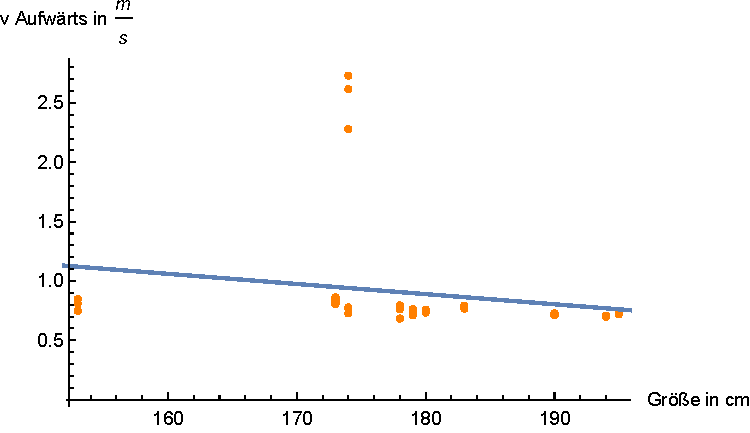
\includegraphics[]{abbildungen/regression/2012/auf-groesse.pdf}
	\[\begin{array}{l|llll}
 \text{} & \text{Estimate} & \text{Standard Error} & \text{t-Statistic} & \text{P-Value} \\
\hline
 1 & 1.42188 & 0.660147 & 2.15388 & 0.0335816 \\
 \text{gr{\" o}{\ss}e} & -0.00301832 & 0.0037105 & -0.813455 & 0.417834 \\
\end{array}\]


	\caption{Abhängigkeit Körpergröße zur Treppengeschwindigkeit aufwärts. Messdaten (orange) mit ermittelter Regressionsgerade (blau). \label{fig:auf2012-groesse}}
\end{figure}

\begin{figure} \centering 
	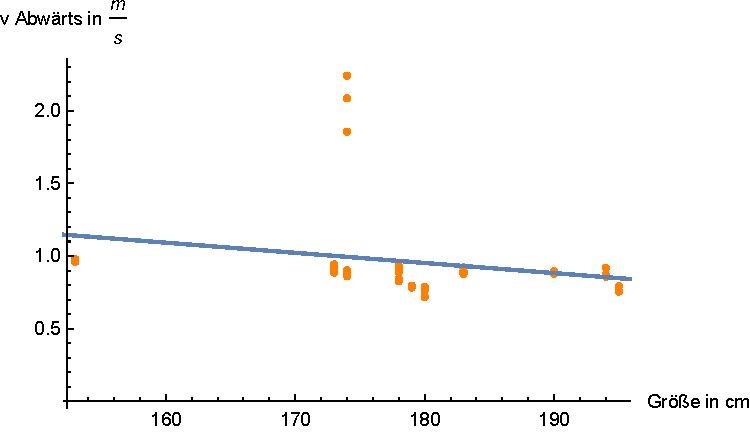
\includegraphics[]{abbildungen/regression/2012/ab-groesse.pdf}
	\[\begin{array}{l|llll}
 \text{} & \text{Estimate} & \text{Standard Error} & \text{t-Statistic} & \text{P-Value} \\
\hline
 1 & 1.59558 & 0.582855 & 2.73753 & 0.00800578 \\
 \text{gr{\" o}{\ss}e} & -0.00253145 & 0.00328881 & -0.769715 & 0.444301 \\
\end{array}\]


	\caption{Abhängigkeit Körpergröße zur Treppengeschwindigkeit abwärts. Messdaten (orange) mit ermittelter Regressionsgerade (blau). \label{fig:ab2012-groesse}}
\end{figure}

Ergebnisse der Plausibilisierung für den Aufstieg 
(Abbildung \ref{fig:auf2012-groesse}):
Signifikanz liegt nicht vor, weil $p > \alpha$. Man nimmt die
Nullhypothese an. Kein Einfluss von $groesse$ auf $v_{auf}$ ist plausibel.

Ergebnisse der Plausibilisierung für den Abstieg
(Abbildung \ref{fig:ab2012-groesse}):
Signifikanz liegt vor, weil $p > \alpha$. Man nimmt die
Nullhypothese an. Kein Einfluss von $groesse$ auf $v_{ab}$ ist plausibel.


\subsubsection{Rundennummer}


Für die Abhängigkeit Rundennummer wurde 
der Zusammenhang (\ref{eq:auf2012-runde}) und (\ref{eq:ab2012-runde}) ermittelt.

\begin{equation} \label{eq:auf2012-runde}
v_{auf}(runde) = 0.940079 - 0.0241206 runde
\end{equation}
\begin{equation} \label{eq:ab2012-runde}
v_{ab}(runde) = 0.940079 + 0.0103279 runde
\end{equation}

In den Abbildungen \ref{fig:auf2012-runde} und \ref{fig:ab2012-runde} ist 
zu sehen, dass sich nach dem Modell die Treppengeschwindigkeit bei Änderung der Runde fast nicht ändert. 

\begin{figure} \centering 
	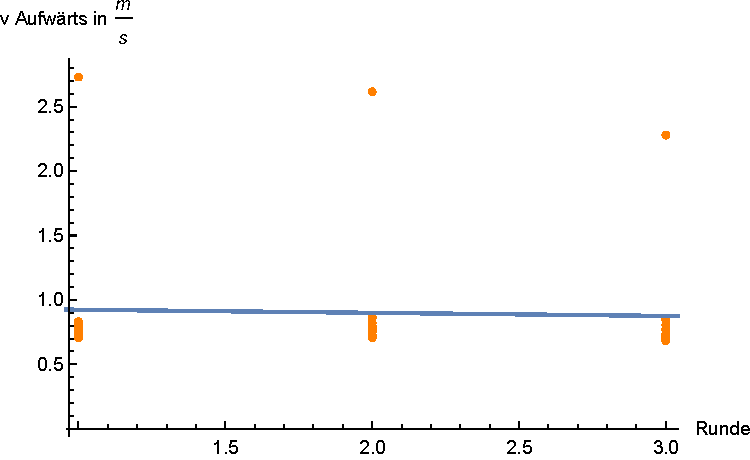
\includegraphics[]{abbildungen/regression/2012/auf-runde.pdf}
	\[\begin{array}{l|llll}
 \text{} & \text{Estimate} & \text{Standard Error} & \text{t-Statistic} & \text{P-Value} \\
\hline
 1 & 0.94804 & 0.2081 & 4.55569 & 0.0000551454 \\
 \text{runde} & -0.0241206 & 0.0963317 & -0.250391 & 0.80367 \\
\end{array}\]


	\caption{Abhängigkeit Rundennummer zur Treppengeschwindigkeit aufwärts. Messdaten (orange) mit ermittelter Regressionsgerade (blau). \label{fig:auf2012-runde}}
\end{figure}

\begin{figure} \centering 
	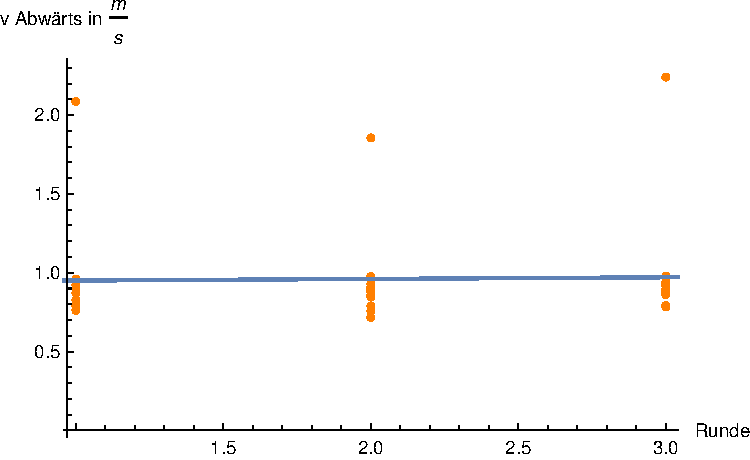
\includegraphics[]{abbildungen/regression/2012/ab-runde.pdf}
	\[\begin{array}{l|llll}
 \text{} & \text{Estimate} & \text{Standard Error} & \text{t-Statistic} & \text{P-Value} \\
\hline
 1 & 0.859522 & 0.0289618 & 29.6777 & \text{6.817362585804904$\grave{ }$*${}^{\wedge}$-26} \\
 \text{runde} & 0.00475595 & 0.0134067 & 0.354744 & 0.724973 \\
\end{array}\]


	\caption{Abhängigkeit Rundennummer zur Treppengeschwindigkeit abwärts. Messdaten (orange) mit ermittelter Regressionsgerade (blau). \label{fig:ab2012-runde}}
\end{figure}

Ergebnisse der Plausibilisierung für den Aufstieg
(Abbildung \ref{fig:auf2012-runde}):
Signifikanz liegt nicht vor, weil $p > \alpha$. Man nimmt die
Nullhypothese an. Kein Einfluss von $runde$ auf $v_{auf}$ ist plausibel.

Ergebnisse der Plausibilisierung für den Abstieg
(Abbildung \ref{fig:ab2012-runde}):
Signifikanz liegt vor, weil $p > \alpha$. Man nimmt die
Nullhypothese an. Kein Einfluss von $runde$ auf $v_{ab}$ ist plausibel.

\subsection{Mehrere Abhängigkeiten}

Hier werden weitere vier lineare Gleichungen mit mehreren Parametern ermittelt.

\[v_{auf}(v_{ebene}, groesse) = \beta_0 + \beta_1 v_{ebene} + \beta_2 groesse\]
\[v_{ab}(v_{ebene}, groesse) = \beta_0 + \beta_1 v_{ebene} + \beta_2 groesse\]

\[v_{auf}(v_{ebene}, groesse, runde) = \beta_0 + \beta_1 v_{ebene} + \beta_2 groesse + \beta_3 runde\]
\[v_{ab}(v_{ebene}, groesse, runde) = \beta_0 + \beta_1 v_{ebene} + \beta_2 groesse + \beta_3 runde\]

Für die Plausibilisierung der Regression wird die Nullhypothese 
$H_0: \beta_1 = 0  \lor \beta_2 = 0$ bzw. $H_0: \beta_1 = 0  \lor \beta_2 = 0 \lor \beta_3 = 0$ aufgestellt.

\subsubsection{Ebenengeschwindigkeit und Größe}

Für die Abhängigkeiten Wunschgeschwindigkeit in der Ebene und Körpergröße wurde 
der Zusammenhang (\ref{eq:auf2012-ebene-groesse}) und (\ref{eq:ab2012-ebene-groesse}) ermittelt.

\begin{equation} \label{eq:auf2012-ebene-groesse}
	v_{auf}(v_{ebene}, groesse) = -2.23812 7 + 1.93153 v_{ebene} + 0.000532946 groesse
\end{equation}
\begin{equation} \label{eq:ab2012-ebene-groesse}
	v_{auf}(v_{ebene}, groesse) = -0.860154 + 1.27065 v_{ebene} + -0.00101083 groesse
\end{equation}

In den Abbildungen \ref{fig:auf2012-ebene-groesse} und \ref{fig:ab2012-ebene-groesse} ist 
zu sehen, dass ein größerer Proband mit schnellerer Ebenengeschwindigkeit auch eine schnellere Treppengeschwindigkeit aufwärts erreicht. Eine schnellere Treppengeschwindigkeit abwärts wird durch einen Proband mit schnellerer Ebenengeschwindigkeit und kleinerer Größe erreicht. Eine Änderung von $50 cm$ in der Größe wirkt sich auf das Besteigen aufwärts mit ca. $0.025 m/s$ und abwärts mit ca. $0.05 m/s$ aus.

\begin{figure} \centering 
	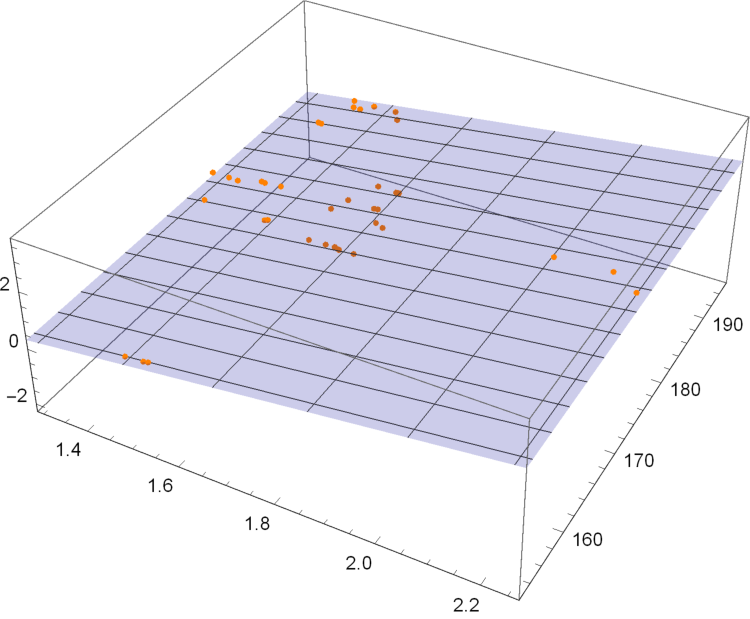
\includegraphics[]{abbildungen/regression/2012/auf-ebene-groesse.pdf}
	\[\begin{array}{l|llll}
 \text{} & \text{Estimate} & \text{Standard Error} & \text{t-Statistic} & \text{P-Value} \\
\hline
 1 & 1.0165 & 0.140132 & 7.25384 & \text{1.5820003769083974$\grave{ }$*${}^{\wedge}$-10} \\
 \text{vEbene} & 0.199894 & 0.0433176 & 4.61461 & 0.0000134806 \\
 \text{gr{\" o}{\ss}e} & -0.00294506 & 0.000643082 & -4.5796 & 0.0000154292 \\
\end{array}\]


	\caption{Abhängigkeiten Ebenengeschwindigkeit und Größe zur Treppengeschwindigkeit aufwärts. Messdaten (orange) mit ermittelter Regressionsebene (blau). \label{fig:auf2012-ebene-groesse}}
\end{figure}

\begin{figure} \centering 
	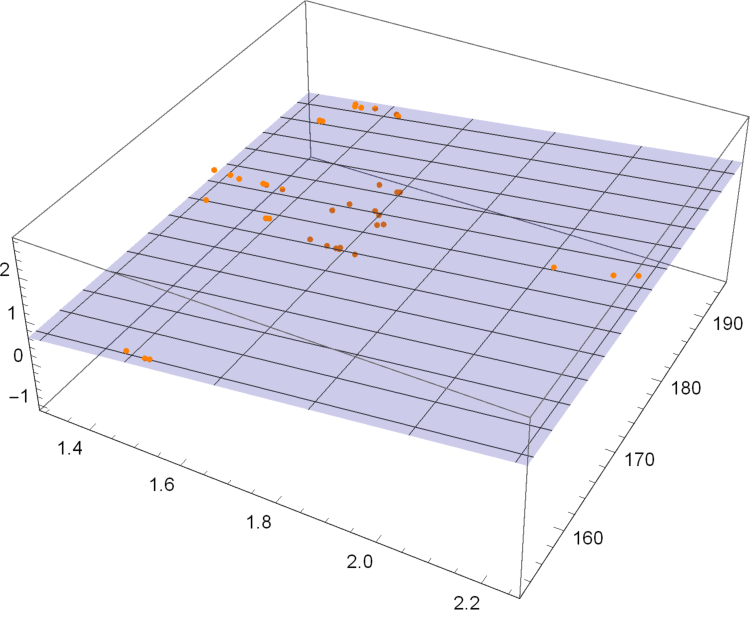
\includegraphics[]{abbildungen/regression/2012/ab-ebene-groesse.pdf}
	\[\begin{array}{l|llll}
 \text{} & \text{Estimate} & \text{Standard Error} & \text{t-Statistic} & \text{P-Value} \\
\hline
 1 & 0.701775 & 0.543236 & 1.29184 & 0.199331 \\
 \text{vEbene} & 0.696676 & 0.127843 & 5.44946 & \text{3.523565756565165$\grave{ }$*${}^{\wedge}$-7} \\
 \text{gr{\" o}{\ss}e} & -0.00382545 & 0.00268911 & -1.42257 & 0.157912 \\
\end{array}\]


	\caption{Abhängigkeiten Ebenengeschwindigkeit und Größe zur Treppengeschwindigkeit abwärts. Messdaten (orange) mit ermittelter Regressionsebene (blau). \label{fig:ab2012-ebene-groesse}}
\end{figure}

Ergebnisse der Plausibilisierung für den Aufstieg
(Abbildung \ref{fig:auf2012-ebene-groesse}):
Signifikanz liegt nicht vor, weil $p_{\beta_2} > \alpha$. Man nimmt die
Nullhypothese an. Kein Einfluss von $v_{ebene}$ und $groesse$ auf $v_{auf}$ ist plausibel.

Ergebnisse der Plausibilisierung für den Abstieg
(Abbildung \ref{fig:ab2012-ebene-groesse}):
Signifikanz liegt nicht vor, weil $p_{\beta_2} > \alpha$. Man nimmt die
Nullhypothese an. Kein Einfluss von $v_{ebene}$ und $groesse$ auf $v_{ab}$ ist plausibel.


\subsubsection{Ebenengeschwindigkeit, Größe und Rundennummer}

Für die Abhängigkeiten Wunschgeschwindigkeit in der Ebene, Körpergröße und Rundennummer wurde 
der Zusammenhang (\ref{eq:auf2012-ebene-groesse-runde}) und (\ref{eq:ab2012-ebene-groesse-runde}) ermittelt.

\begin{multline} \label{eq:auf2012-ebene-groesse-runde}
v_{auf}(v_{ebene}, groesse, runde) = \\
-2.20269 + 1.93049 v_{ebene} + 0.000528021 groesse - 0.0164501  runde
\end{multline}
\begin{multline} \label{eq:ab2012-ebene-groesse-runde}
v_{auf}(v_{ebene}, groesse, runde) = \\
- 0.893281 + 1.27163 v_{ebene} - 0.00100623 groesse + 0.0153806  runde
\end{multline}

\begin{figure} \centering 
	\[\begin{array}{l|llll}
 \text{} & \text{Estimate} & \text{Standard Error} & \text{t-Statistic} & \text{P-Value} \\
\hline
 1 & 1.01208 & 0.137206 & 7.37634 & \text{2.1703587613814404$\grave{ }$*${}^{\wedge}$-8} \\
 \text{vEbene} & 0.117482 & 0.0493951 & 2.37842 & 0.0235248 \\
 \text{gr{\" o}{\ss}e} & -0.00231594 & 0.000542029 & -4.27274 & 0.000161828 \\
 \text{runde} & -0.00663057 & 0.00696761 & -0.951628 & 0.348419 \\
\end{array}\]


	\caption{Abhängigkeiten Ebenengeschwindigkeit, Größe und Runde zur Treppengeschwindigkeit aufwärts.
	\label{fig:auf2012-ebene-groesse-runde}}
\end{figure}

\begin{figure} \centering 
	\[\begin{array}{l|llll}
 \text{} & \text{Estimate} & \text{Standard Error} & \text{t-Statistic} & \text{P-Value} \\
\hline
 1 & 1.54231 & 0.231512 & 6.66191 & \text{1.6207125042011794$\grave{ }$*${}^{\wedge}$-7} \\
 \text{vEbene} & -0.070368 & 0.083346 & -0.844287 & 0.404777 \\
 \text{gr{\" o}{\ss}e} & -0.00320726 & 0.000914584 & -3.5068 & 0.00136734 \\
 \text{runde} & 0.0043198 & 0.0117567 & 0.367433 & 0.715715 \\
\end{array}\]


	\caption{Abhängigkeiten Ebenengeschwindigkeit, Größe und Runde zur Treppengeschwindigkeit abwärts.
	\label{fig:ab2012-ebene-groesse-runde}}
\end{figure}

Ergebnisse der Plausibilisierung für den Aufstieg
(Abbildung \ref{fig:auf2012-ebene-groesse-runde}):
Signifikanz liegt nicht vor, weil $p_{\beta_2} > \alpha$ und $p_{\beta_3} > \alpha$. Man nimmt die Nullhypothese an.

Ergebnisse der Plausibilisierung für den Abstieg
(Abbildung \ref{fig:ab2012-ebene-groesse-runde}):
Signifikanz liegt nicht vor, weil $p_{\beta_2} > \alpha$ und $p_{\beta_3} > \alpha$. Man nimmt die Nullhypothese an.